\documentclass[10pt, oneside, a4paper]{article}
\usepackage{ifpdf}
\usepackage{graphicx}
\usepackage[colorlinks,bookmarksopen,linkcolor=black,pdfauthor={Vikram},urlcolor=blue]{hyperref}
\usepackage[colorlinks,bookmarksopen]{hyperref}
\usepackage[hmargin=1.5cm,vmargin=2.5cm]{geometry}
\usepackage{amsmath}
\usepackage{algorithmic}
\usepackage{algorithm}
\begin{document}
\begin{center}
\textbf{VISVESWARAYA TECHNOLOGICAL UNIVERSITY}
\end{center}
\begin{center}
\textbf{BELGAUM}\\
\thispagestyle{empty}
\begin{figure}[htb]
\begin{center}
\ifpdf

\includegraphics[scale=0.50]{vtu.png}
\else
\fi
\end{center}
\end{figure}
\textbf{SRI JAYACHAMARAJENDRA COLLEGE OF ENGINEERING,}
\textbf{MYSORE-570006}\\
\textsc{department of computer science and engineering}
\end{center}
\begin{figure}[htb]
\begin{center}
\ifpdf

\includegraphics[scale=0.30]{./logo.png}
\else
\fi
\end{center}
\end{figure}
\begin{center}
\textbf{\underline{Report on}}\\
\textsc{\\IMPLEMENTATION OF STATIC SINGLE-ASSIGNMENT (SSA) FORM\\}
\emph{\\Guidance of}\\
\textbf{\\N.R. PRASHANTH}\\
\textit{Professor}\\
\textit{Department of CS$\&$E, SJCE, Mysore.}\\
\vspace{1in}
\textbf{\underline{Done By:}}\\
\textsc{\\VIKRAM T.V.}\\
5th Semester,\\ Computer Science and Engineering,\\
S.J.C.E, Mysore\\
\title {IMPLEMENTATION OF STATIC SINGLE-ASSIGNMENT (SSA) FORM\\}
\end{center}
\newpage
\thispagestyle{empty}
\tableofcontents
\newpage
\pagenumbering{arabic}

\twocolumn
\section{Introduction}
Data flow analysis needs the \emph{def-use} chain to find the use-sites of each defined variable or the def-sites of each variable used in an expression.  An improvement on the idea of def-use chains is \emph{static single-assignment form}, or SSA form, which is an intermediate form in which each variable has only one definition in the program text.  The static definition-site may be in a loop that is executed many times, thus the name - static single assignment form, where the variables are never redefined.  Some of the advantages of using SSA form are: optimizations and dataflow analysis becomes simpler, space complexity reduces compared to def-use chains and unrelated uses of same variable (inside a loop) in source program become different in SSA form, eliminating needless relationships.

\begin{figure}[htb]
\begin{center}
\ifpdf
	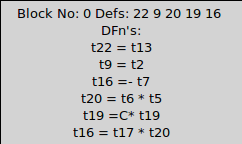
\includegraphics[scale=0.50]{./straightLineProgram.png}
\else
\fi
\caption{A straight line program}
\label{fig:1}
\end{center}
\end{figure}
\begin{figure}[htb]
\begin{center}
\ifpdf
	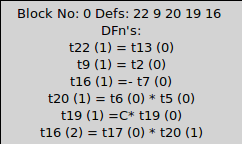
\includegraphics[scale=0.50]{./programInSSa.png}
\else
\fi
\caption{Program in SSA form}
\label{fig:2}
\end{center}
\end{figure}

Figure 1 shows a straight line program and figure 2 shows the corresponding program in SSA form.  When two control flow paths merge together, with each path having a definition of \emph{a} as \emph{a1} (across left path) and \emph{a2} (across right path), it is essential to have only one definition of \emph{a} at the merge point to have the program in SSA form.  A new definition of \emph{a}, say \emph{a3}, is defined at the merged point which is the result of $\phi$-function.  Thus the statement \emph{a3} $\leftarrow$ $\phi$(\emph{a1}, \emph{a2}) defines \emph{a3} with \emph{a1}, if the control flow was through left path, or with \emph{a2} if control flow took right path.  The $\phi$ functions are eliminated before generating executable by placing MOVE instructions on each incoming edge with corresponding definitions.  Figure 3 shows an example of $\phi$ placement for the variable t13.

\begin{figure}[htb]
\begin{center}
\ifpdf
	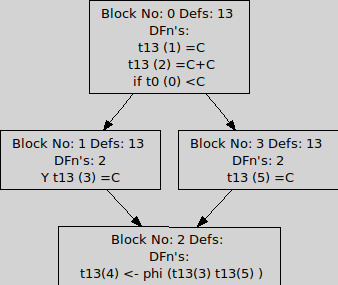
\includegraphics[scale=0.50]{./ssaExample.png}
\else
\fi
\caption{$\phi$-function placement}
\label{fig:3}
\end{center}
\end{figure}

\section{Converting to SSA Form}
Converting a program to SSA form involves 4 stages: creating dominators for each basic block,  find the places where $\phi$ functions have to be placed, placing of $\phi$ functions and finally renaming of uses and definitions of variables.  The input program is the intermediate representation represented using basic blocks and control flow graph.

\subsection{Dominators}
The dominators for the basic blocks of the input program are calculated using the Lenguer-Tarjan algorithm.  An immediate dominator is found for each of the nodes.  This is used to find places needed for $\phi$ placement.

\subsection{The Dominance Frontier}
Finding places for $\phi$ placement can be calculated iteratively.  The criterion for this is to find a blocks \emph{x} and \emph{y} (with \emph{x} $\neq$ \emph{y}) containing definitions of \emph{a}.  A $\phi$ function should be at node \emph{z}, if there are non-empty paths P$_\emph{x}$$_\emph{z}$ and P$_\emph{y}$$_\emph{z}$ and both paths do not have any node in common other than \emph{z}.  Also node \emph{z} does not appear within both paths.  But we can use the dominance properties on SSA form to find a better method of placing $\phi$ functions, known as the Dominance Frontier criterion, which relies on following properties:

\begin{itemize}
\item If \emph{x} is used in a $\phi$-function in block \emph{n}, then the definition of \emph{x} dominates every predecessor of \emph{n}.
\item If \emph{x} is used in a non-$\phi$-statement in block \emph{n}, then the definition of \emph{x} dominates \emph{n}.
\end{itemize}

The dominance frontier is calculated using the dominator tree of the flow graph.  \emph{x strictly dominates w} if \emph{x} dominates \emph{w} and \emph{x} $\neq$ \emph{w}.  A dominance frontier of a node \emph{x} is the set of all nodes \emph{w} such that \emph{x} dominates a predecessor of \emph{w}, but does not strictly dominate \emph{w}.  A dominance frontier of a node is the border between the dominated and undominated nodes, and it is here the $\phi$-functions have to be placed.  Hence, the criterion is: whenever node \emph{x} contains a definition of some variable \emph{a}, then any node \emph{z} in the dominance frontier of \emph{x} needs a $\phi$-function for \emph{a}.

\textbf{Computing the dominance frontier}:  To insert all the necessary $\phi$-functions, for every node \emph{n} in the flow graph, DF[n] is needed, its dominance frontier, which can be computed efficiently in one pass using the dominator tree.  The following sets are used:

\begin{itemize}
\item DF$_{local}$[n]:  The successors of \emph{n} that are not strictly dominated by \emph{n}.
\item DF$_{up}$[n]:  Nodes in the dominance frontier of \emph{n} that are not strictly dominated by \emph{n}'s immediate dominator.
\end{itemize}

\begin{algorithm}
\caption{Psuedocode for computeDF[\emph{n}]}
\label{alg1}
\begin{algorithmic}[1]
\STATE \textbf{computeDF[\emph{n}] ( )}
\STATE S $\leftarrow$ $\{$ $\}$
\FOR {each node \emph{y} in \emph{successor[\emph{n}]}}
\IF {\emph{idom(y)} $\neq$ \emph{n}}
\STATE S $\leftarrow$ S $\cup$ {\emph{y}}
\ENDIF
\ENDFOR
\FOR {each child \emph{c} of \emph{n} in the dominator tree}
\STATE computeDF[\emph{c}]
\FOR {each element \emph{w} of DF[\emph{c}]}
\IF {\emph{n} does not dominate \emph{w} or \emph{n} = \emph{w}}
\STATE S $\leftarrow$ S $\cup$ {\emph{w}}
\ENDIF
\ENDFOR
\ENDFOR
\STATE DF[\emph{n}] $\leftarrow$ S
\end{algorithmic}
\end{algorithm}

The dominance frontier of \emph{n} can be computed from DF$_{local}$ and DF$_{up}$:\\\\
DF[n] = DF$_{local}$[n] $\bigcup$ $\cup_{\substack{c{\in}children[n]}}$ DF$_{up}$[\emph{c}]\\\\
where children[n] are the nodes whose immediate dominator is \emph{n}.  Using immediate dominators DF$_{local}$[n] is calculated as the set of those successors of \emph{n} whose immediate dominator is not \emph{n}.  A pseudocode to compute DFn is given in Algorithm 1.  Its complexity is proportional to the number of edges of the original graph plus the size of the dominance frontiers it computes.  But practically, the control flow graphs for the programs are not that complex and hence this psuedocode runs in linear time.

\subsection{Inserting $\phi$-functions}
A pseudocode for inserting $\phi$-functions is shown in Algorithm 2.  It uses worklists to avoid reexamining of nodes where no $\phi$-function has been inserted.  First the definition sites of the variables in each block is computed.  A$_{orig}$[n] contains the variable definitions at node \emph{n}.  A$_{\phi}$[n] gives the variables that have $\phi$-functions at node \emph{n}.  Y contains a dominance frontier of node \emph{n}.  For each variable \emph{a}, the definition sites of \emph{a} are loaded into the worklist.  For each node \emph{n} in the worklist, until the worklist becomes empty,  for each node in DF[\emph{n}], if variable \emph{a} is not in A$_{\phi}$[n], then insert the statement a $\leftarrow$ $\phi$(a, a, ..., a) at the top of block Y, where $\phi$-function has as many arguments as Y has predecessors.  Add the variable \emph{a} to A$_{\phi}$[Y] and check if \emph{a} is not in A$_{orig}$[n], that is if there is no definition of \emph{a}, then add the current node into the worklist.

\begin{algorithm}
\caption{Psuedocode for Inserting $\phi$-functions}
\label{alg2}
\begin{algorithmic}[1]
\STATE \textbf{Place-$\phi$-functions ( )}
\FOR {each node \emph{n}}
\FOR {each variable \emph{a} in A$_{orig}$[\emph{n}]}
\STATE \emph{defsites}[a] $\leftarrow$ \emph{defsites}[a] $\cup$ {\emph{n}]}
\ENDFOR
\ENDFOR
\FOR {each variable \emph{a}}
\STATE W $\leftarrow$ \emph{defsites}[\emph{a}]
\WHILE {W not empty}
\STATE remove some node \emph{n} from W
\FOR {each Y in  DF[\emph{n}]}
\IF {\emph{a} $\notin$ A$_{\phi}$[Y]}
\STATE insert the statement \emph{a} $\leftarrow$ (\emph{a}, \emph{a}, ..., \emph{a}) at the top of block Y, where the $\phi$-function has as many arguments as Y has predecessors
\STATE A$_{\phi}$[Y] $\leftarrow$ A$_{\phi}$[Y] $\cup$ {\emph{a}}
\IF {\emph{a} $\notin$ A$_{orig}$[\emph{n}]}
\STATE W $\leftarrow$ W $\cup$ {Y}
\ENDIF
\ENDIF
\ENDFOR
\ENDWHILE
\ENDFOR
\end{algorithmic}
\end{algorithm}


For a program of size of N, the work done for each node and edge in control flow graph and for each statement in program are proportional to N.  For each element of every dominance frontier, the complexity is approximately linear in N and the number of inserted $\phi$-functions could be N$^2$ in worst case, but practically it is proportional to N.  Thus, the algorithm works in linear time.


\subsection{Renaming the Variables}
After $\phi$-function placement, renaming of different definitions (including $\phi$-function definitions) of variable \emph{a} to \emph{a1}, \emph{a2}, \emph{a3} and so on are done using the dominator tree.  Each use of \emph{a} is renamed to use the closest definition of \emph{a} that is above \emph{a} in the dominator tree and this handling is done using separate stack for each variable.  For each statement S in each block \emph{n}, if the statement is not a $\phi$-function then replace each use of the statement with its latest definition.  That is replace the use \emph{x} with \emph{x$_i$}, where \emph{i} denotes the latest definition of \emph{x}.  For each definition in each statement (including the $\phi$-functions, increment the count of the new definition and push it (\emph{i}) onto corresponding stack.  Replace definition of \emph{a} with \emph{a$_i$}.  For each successor Y of block \emph{n}, if \emph{n} is the \emph{j}th predecessor of Y, then replace the \emph{j}th use of variable \emph{a} in $\phi$-function at block \emph{n} with \emph{a$_i$}, where \emph{i} is the latest defined value of \emph{a}.  A psuedocode is given in algorithm 3.

\begin{algorithm}
\caption{Psuedocode for Renaming Variables}
\label{alg3}
\begin{algorithmic}[1]
\STATE \textbf{initialize ( )}
\FOR {each variable \emph{a}}
\STATE count[\emph{a}] $\leftarrow$ 0
\STATE stack[\emph{a}] $\leftarrow$ empty
\STATE push 0 onto stack[\emph{a}]
\ENDFOR

\STATE \textbf{rename (\emph{n})}
\FOR {each statement S in block \emph{n}}
\IF {S is not a $\phi$-function}
\FOR {each use of some variable \emph{x} in S}
\STATE \emph{i} $\leftarrow$ top(stack[\emph{x}])
\STATE replace the use of \emph{x} with \emph{x$_i$} in S
\ENDFOR
\ENDIF
\FOR {each definition of some variable \emph{a} in S}
\STATE count[\emph{a}] $\leftarrow$ count[\emph{a}] + 1
\STATE \emph{i} $\leftarrow$ count[\emph{a}]
\STATE push \emph{i} onto stack[\emph{a}]
\STATE replace definition of \emph{a} with definition of \emph{a$_i$} in S
\ENDFOR
\ENDFOR
\FOR {each successor Y of block \emph{n}}
\STATE suppose \emph{n} is the \emph{j}th predecessor of Y
\FOR {each $\phi$-function in Y}
\STATE suppose the \emph{j}th operand of the $\phi$-function is \emph{a}
\STATE \emph{i} $\leftarrow$ top(stack[\emph{a}])
\STATE replace the \emph{j}th operand with \emph{a$_i$}
\ENDFOR
\ENDFOR
\FOR {each child X of \emph{n}}
\STATE rename(X)
\ENDFOR
\FOR {each definition of some variable \emph{a} in the original S}
\STATE pop stack[\emph{a}]
\ENDFOR
\end{algorithmic}
\end{algorithm}

This algorithm takes time proportional to the size of the program (after $\phi$-functions are inserted), so in practice the algorithm runs in linear time.  Finally, if the Lenguer-Tarjan algorithm is implemented efficiently with approximate linear complexity, then all the four stages of SSA works in around linear time, making the whole SSA implementation to work in linear time.

\section{Some examples}
Figure 3 shows the control flow graph after $\phi$-function placement at node 2 for variable t13.  Variable t13 is defined along both the paths of the if-else construct - once along the 'if' path and along 'else' path.  Thus, there needs a $\phi$-function at the convergence of the two paths - node 2.  All the figures show the node or block numbers, variables defined in the corresponding block and the DF[node].  In the above example, DF[1] is 2, which means there needs to be a $\phi$-function placement at node 2.

\begin{figure}[htb]
\begin{center}
\ifpdf
	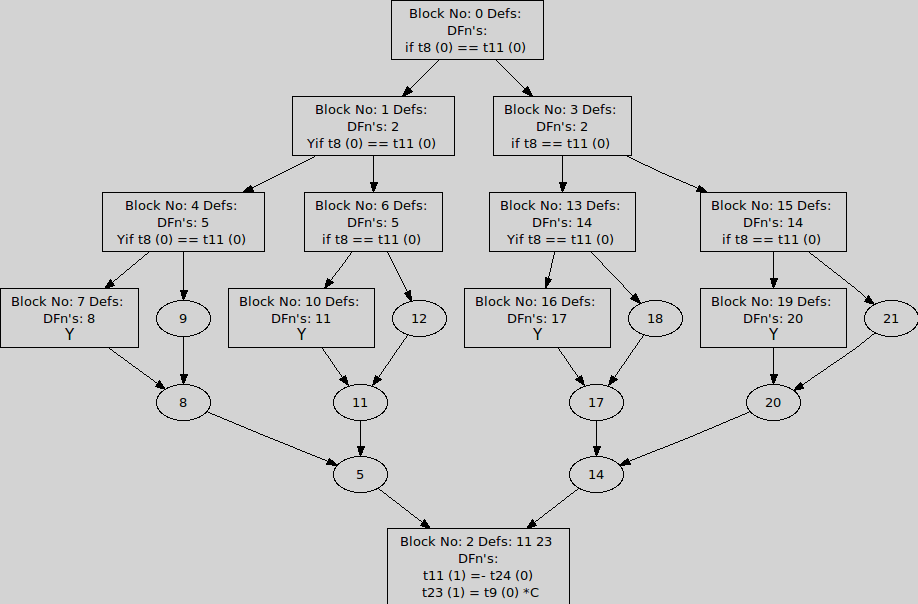
\includegraphics[scale=0.35]{./ifelse.png}
\else
\fi
\caption{A complex if-else construct}
\label{fig:4}
\end{center}
\end{figure}

Figure 4 shows the graph for a complex if-else construct with no necessity of $\phi$-function placement and figure 5 shows $\phi$-function placement for a simple loop.

\begin{figure}[htb]
\begin{center}
\ifpdf
	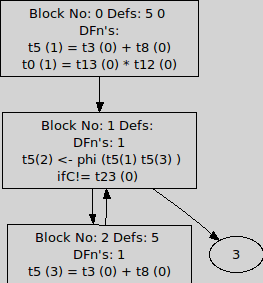
\includegraphics[scale=0.50]{./loop.png}
\else
\fi
\caption{$\phi$-function placement for a loop}
\label{fig:5}
\end{center}
\end{figure}

\begin{thebibliography}{10}
\bibitem {appel}{appel} andrew w. appel, \emph{modern compiler implementation in c}, Revised Edition, Cambridge University Press, 2008
\end{thebibliography}

\end{document}